\documentclass[12pt]{article}
\usepackage[utf8]{inputenc}
\usepackage{listings}
\usepackage{amsmath, amssymb}
\usepackage{braket}
\usepackage[margin=1.3in]{geometry}

\title{IBM Quantum Experience Review}
\author{Boettner, Neumann, Gopalan}
\date{May 2020}

\usepackage{subfigure}
\usepackage{xcolor}
\usepackage{graphicx}
\usepackage{float}

\linespread{1.25}

\definecolor{codegreen}{rgb}{0,0.6,0}
\definecolor{codegray}{rgb}{0.5,0.5,0.5}
\definecolor{codepurple}{rgb}{0.58,0,0.82}

\lstdefinestyle{qasm}{
    commentstyle=\color{codegreen},
    keywordstyle=\color{magenta},
    numberstyle=\tiny\color{codegray},
    stringstyle=\color{codepurple},
    basicstyle=\ttfamily\footnotesize,
    breakatwhitespace=false,         
    breaklines=true,                 
    captionpos=b,                    
    keepspaces=true,                 
    numbers=left,                    
    numbersep=5pt,                  
    tabsize=2
}

\lstset{style=qasm}
\newcommand{\url}{\footnote{https://quantum-computing.ibm.com/docs/circ-comp/q-gate}} % too long for body
\newcommand{\qasm}{\footnote{https://github.com/Qiskit/openqasm}}
\newcommand{\ibm}{\footnote{https://thequantumdaily.com/2020/01/30/getting-real-time-information-on-ibm-quantum-devices/}}
\begin{document}

\maketitle

\section{The IBM Q System One}
    
    \begin{figure}[h!]
        \centering
        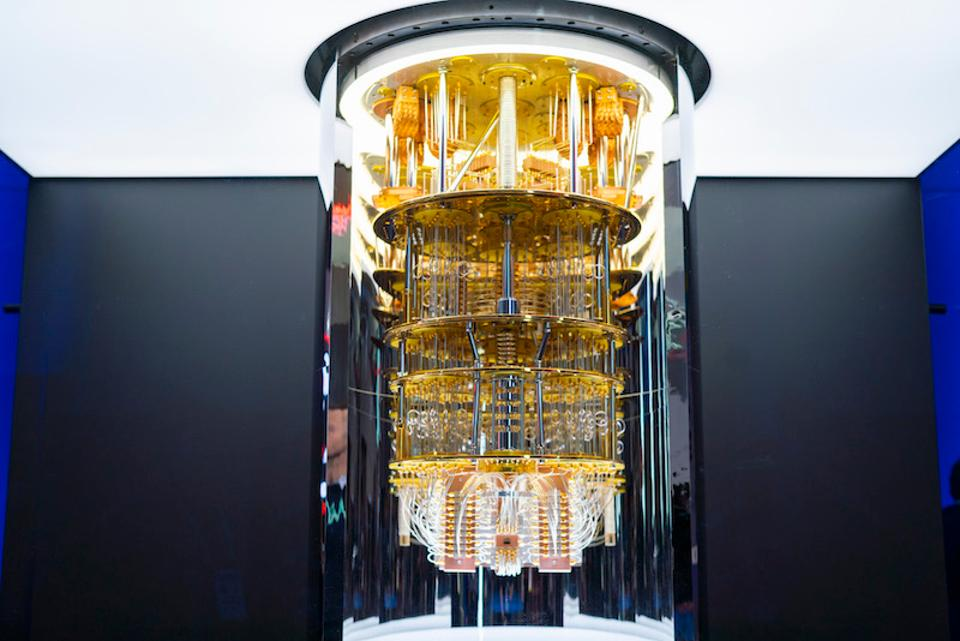
\includegraphics[width=\linewidth]{Circuits/ibm-q.jpg}
        \caption{The IBM Q System One quantum computer}
    \end{figure}
    
    \noindent
    All computing systems rely on a fundamental ability to store and manipulate information. Classical computers manipulate individual bits, which store information as binary 0 and 1 states. Quantum computers instead leverage quantum mechanical phenomena to manipulate information. To do this, they rely on quantum bits, or qubits, which are unit vectors in $\mathbb{C}^2$. Storing and manipulating data in the form of qubits leads to more information, which allows for several fast and efficient algorithms for tasks that are harder or impossible to solve on a classical computer.
    \\
    \smallskip
    \\
    The history of quantum computing research goes all the way back to 1927 and each result marked a new piece of the puzzle. In October 2017, a significant mathematical result was published in the paper “Quantum Advantage with Shallow Circuits” (Bravyi et al. 2018), which guided the development of algorithms for quantum computing. The significance of this algorithm was that unlike Shor’s algorithm, it proved that a quantum computer can solve certain problems with near certainty in a fixed number of steps, no matter the increased input. A classical computer, on the other hand,  would require an increased number of steps as the input increases for the same problems. This made the Quantum Advantage algorithm a solid and necessary brick in the foundation of quantum computing.
    \\
    \smallskip
    \\
    Building on this foundation, in 2019 IBM Quantum designed and built the world’s first integrated quantum computing system for commercial use: IBM Q System One\ibm\,in order to make quantum computers more reliable and stable. IBM Q System One enabled universal approximate superconducting quantum computers to operate beyond the confines of the research lab and is available online for free. In this paper, we recreate circuits to experiment with the Grover’s Search algorithm and the Deutsch-Josza algorithm, and describe both our results as well as what we learned during the process.


\section{Coding in IBM Q}
    \textbf{IBM Q} was designed to make computing the outcome of Quantum circuits as simple as possible. The built in Circuit Composer allows users to intuitively click and drag universal quantum gates onto a set of qubits. The user can then view the \textbf{QASM} language\qasm \ encoding of their circuit and manipulate it further if they wish. Finally, IBM's cloud based compute model allows the user to run their encoding on one of IBM's servers where it will join a queue before the results of the quantum circuit are sent back to the user. This whole process is highly documented and user friendly. 
    
    This section will outline how to use the Circuit Composer to make and test quantum circuits as well as provide some simple examples of the interface.
    
    \subsection{Circuit Composer}
        The IBM Q Circuit Composer presents the circuit visual as well as the \textbf{QASM} circuit encoding side by side. By allowing interactions with either, this platform helps the user quickly learn how to tweak their circuit exactly as they want it. This visual interface provides icons for each gate along with a glossary entry for each icon that explains what the gate does. Despite providing the option to write code, the Circuit Composer in no way forces the user to have past programming experience. The QASM representation simply allows more precise control over the circuit creation process.
        
        \begin{figure}[ht]
            \centering
            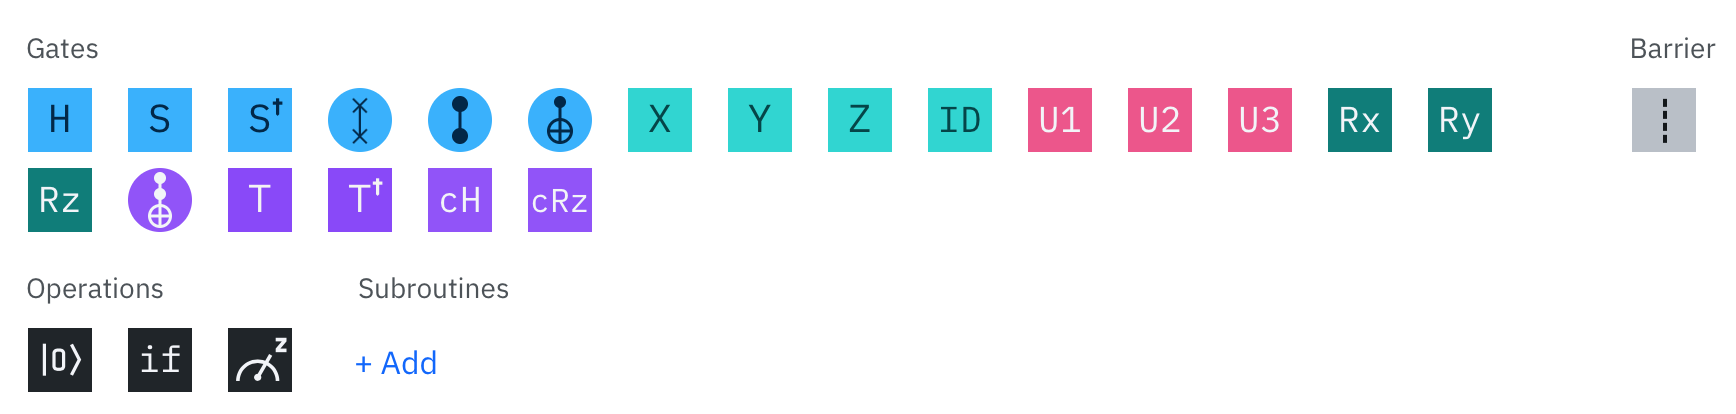
\includegraphics[width=\linewidth]{Circuits/gates.png}
            \caption{Gates in the Circuit Composer}
        \end{figure}
        
    \subsection{Encoding}
        Circuit encoding in IBM Q is simple. The software uses the QASM language developed by IBM in 2017 and uses arrays to represent qubit input states. The QASM provides a set of quantum gates that are represented with letters and take the qubits they are being applied to as inputs. The order in which these appear in the code correlates to the order they appear on the circuit. This encoding can then be interpreted by the IBM servers in order to compute the results of the circuit.
        \\
         \smallskip
        \\
        Encoding each circuit into a small file is a crucial element of IBM Q software for a number of reasons. Most importantly, the simplified and optimized encoding helps combat the severe limitations of our current quantum computing capabilities. The optimization occurs when IBM transpiles\footnote{The transpiler introduces the concept of a pass manager to allow users to explore optimization and find better quantum circuits for their given algorithm (Qiskit 20).} the circuit encoding. In this process, the number of quantum gates is reduced as much as possible while maintaining the circuit's properties. Additionally, the small file size minimizes data transfer between users and IBM servers which allows faster and more convenient access for everyone.

    \subsection{Getting Results}
        As previously mentioned, IBM Q is fully cloud based. This system utilizes multiple global servers to process user circuits. When a user submits their circuit to be run a specified number of times, it joins a server queue. These servers utilize classical computers to decode the quantum circuit and send the corresponding qubits to a real quantum computer. The quantum computer then runs the circuit the set number of times and returns the results from the circuit back to the user. The results use a histogram to display each returned state along with probability with which that state appeared. These results also include the time it took for the circuit to transpile, validate, queue, and run.
        
        
\section{Theory}
    \subsection{Deutsch-Jozsa algorithm}
    
    The Deutsch-Jozsa algorithm was the first to show a separation between the quantum and classical difficulty of a problem. Formally, it is defined as follows: Consider a function $f(x)$ that takes as input $n$-bit strings $x$ and returns 0 or 1, where we are promised that $f(x)$ is either a \emph{constant} function that takes the same value $c \in {0,1}$ on all inputs $x$, or a \emph{balanced} function that takes each value 0 and 1 on exactly half of the inputs. \textbf{The goal is to decide whether $f$ is constant or balanced by making as few function evaluations as possible}. 
    \\
    \smallskip
    \\
    A simple implementation of this was what we did in class, where we used the phase kickback trick for an oracle to guess the sum of two bits using only a single query, which classically would take 2 queries. In our experiments, we implement a more `quantum-like' experimental setup that is described \textbf{here}\footnote{see https://quantum-computing.ibm.com/docs/guide/q-algos/deutsch-jozsa-algorithm}. In this setup, consider a typical interference experiment where a particle that behaves like a wave, such as a photon, can travel from the source to an array of detectors by following two or more paths simultaneously. The probability of observing the particle will be concentrated at those detectors where most of the incoming waves arrive with the same phase. We can set up the $2^n$ possible paths and $2^n$ detectors with $n$-bit strings $x$ and $y$ respectively. Though this experiment is not practical since it would require an impossibly large optical table, we can simulate this experiment on a quantum computer with just $n$ qubits and access to the oracle circuit $U_f$. Classically, this method requires $2^{n-1}+1$ function evaluations in the worst case, but using the Deutsch-Jozsa algorithm the question can be answered with just one function evaluation.
    \\
    \smallskip
    \\
    Suppose that the phase accumulated along a path $x$ to a detector $y$ equals $C(-1)^{f(x)+x.y}$ where $x.y = \sum_{i=1}^{n} x_{i}y_{i}$ is the binary inner product and $C$ is a normalizing coefficient. The probability to observe the particle at a detector $y$ can be computed by summing up amplitudes of all paths $x$ arriving at $y$ and taking the absolute value squared, i.e.,:
    \begin{equation}
        Pr(y) = \mid C\sum_{x}(-1)^{f(x)+x.y} \mid^{2}
    \end{equation}
    
    \noindent
    The normalization condition, $\sum_{y}Pr(y) = 1$, gives us $C = 2^{-n}$. Now, we can compute the probability  of observing the particle at the detector $y = 0^n$ (all zeros string). We have $Pr(y=0^{n}) = \mid2^{-n}\sum_{x}(-1)^{f(x)}\mid^2$. If $f(x) = c$ is a constant function, we get $Pr(y=0^{n}) = \mid(-1)^c\mid^2 = 1$. However, if $f(x)$ is a balanced function, we get $Pr(y=0^{n}) = 0$, since all the terms in the sum over  cancel each other out. We can therefore determine whether $f$ is constant or balanced with certainty by running the experiment just once. This methodology gives us the Deutch-Josza algorithm:
    
    \begin{enumerate}
        \item Initialize $n$ qubits in the all-zeros state $\ket{0,0,\cdots,0}.$
        \item Apply the Hadamard gate $\mbox{\em{H}}$ to each qubit.
        \item Apply the oracle $U_{f}$.
        \item Repeat Step 2.
        \item  Measure each qubit. Let $y = (y_1, \cdots, y_n)$ be the list of measurement outcomes. We find that $f$ is a constant function if $y$ is the all-zeros string.
    \end{enumerate}
    
    \noindent
   The applications of Hadamards at Step 4 maps a basis state  to a superposition $2^{-n/2}\sum_{y}(-1)^{x.y}\ket{y}$. Thus the state reached after Step 4 is $\ket{\Psi} = \sum_{y}\Psi(y)\ket{y}$, where $\Psi (y) = 2^{-n}\sum_{x}(-1)^{f(x)+x.y}$. This is exactly what we need for the interference experiment described above. The final measurement at Step 5 plays the role of detecting the particle. The probability to measure  at Step 5 is 1 if $f$ is a constant function and 0 if $f$ is a balanced function. Thus we have solved the Deutsch-Jozsa problem with certainty by making just one function evaluation.
    
    
    
    \subsection{Grover Search algorithm}
    
    
    
        
\section{Expressing Circuits in IBM Q}
    To show how QASM and IBM Q works we took two examples from class and tested the QASM implementation against their known results. For both Deutsch-Jozsa and Grover Search IBM included numerous examples and we decided to test these examples to see if they held up to their theoretical results. While we did learn how encode circuits in QASM, using the examples allows us to test IBM's implementations and makes sure there are no errors in our encoding. These examples were run multiple times through the IBM server and we made sure they encoded the proper algorithms. The subsections bellow detail our results.
    
    \subsection{Deutsch-Jozsa algorithm}
        For this example we tested a constant and balanced function with the Deutsch-Jozsa algorithm. IBM's example for a balanced function over three qubits uses Hadamard gates, a C-not and a controlled Z-gate. This function should never return the all zero state. In contrast the constant function just Hadamards each qubit twice with no function in the middle (this is clearly a constant function as it is the Deutsch-Jozsa of the trivially constant function). When the first example circuit is run through the IBM Q software it returned even results for each state, but the all zero qubit state. This suggests that the function is balanced as the Deutsch-Jozsa algorithm never returns the string of all zeros. In contrast for the trivial constant function, the result was always the state of all zero qubits. This clearly shows that the software correctly evaluated both example circuits. We ran these simulations multiple times and never had any errors or false positives demonstrating that the quantum computer always correctly evaluated the circuits.
        \begin{figure}[ht]
            \centering
            \begin{minipage}{0.35\linewidth}
                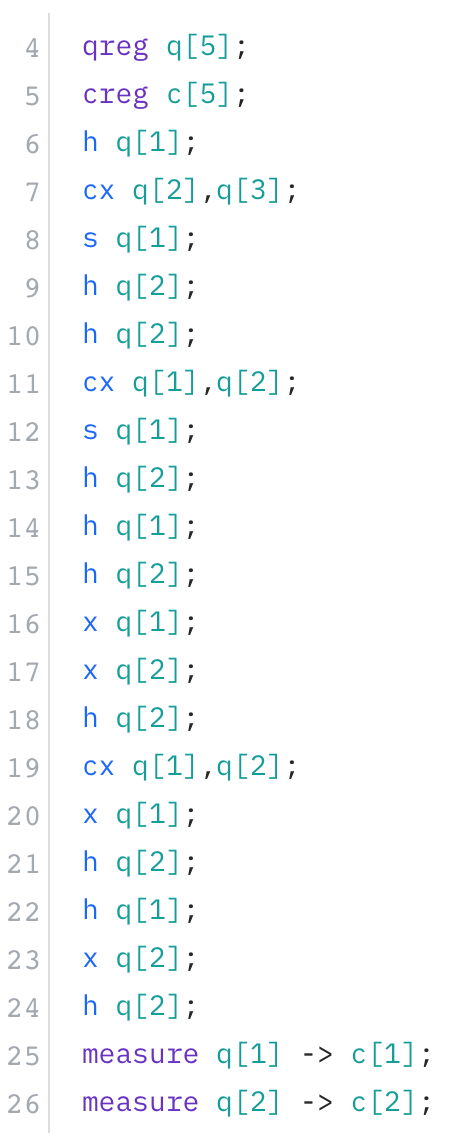
\includegraphics[width=\linewidth]{Circuits/Deutsch-Jozsa-code.png}
            \end{minipage}%
            \begin{minipage}{0.65\linewidth}
                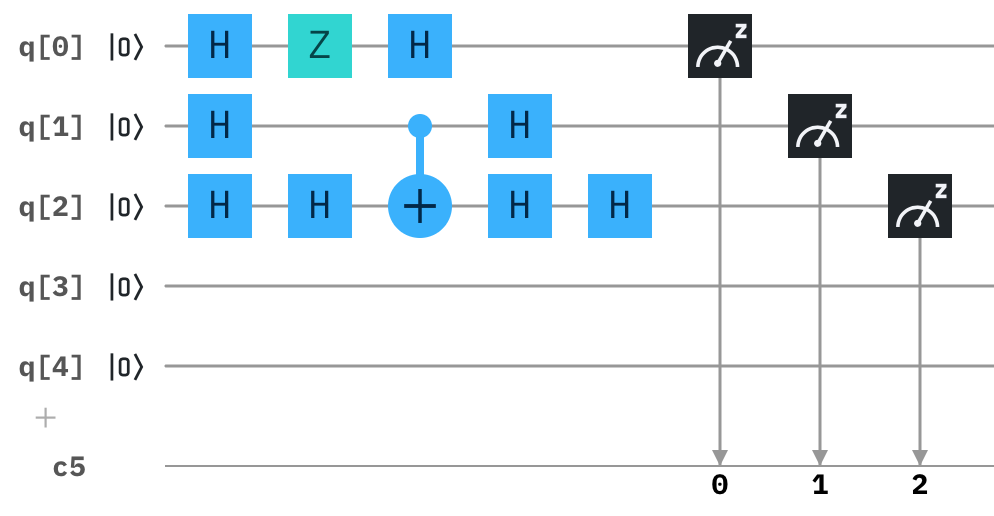
\includegraphics[width=\linewidth]{Circuits/Deutsch-Jozsa.png}
            \end{minipage}
            \caption{Deutsch-Jozsa algorithm}
        \end{figure}
        \begin{figure}[ht]
            \centering
            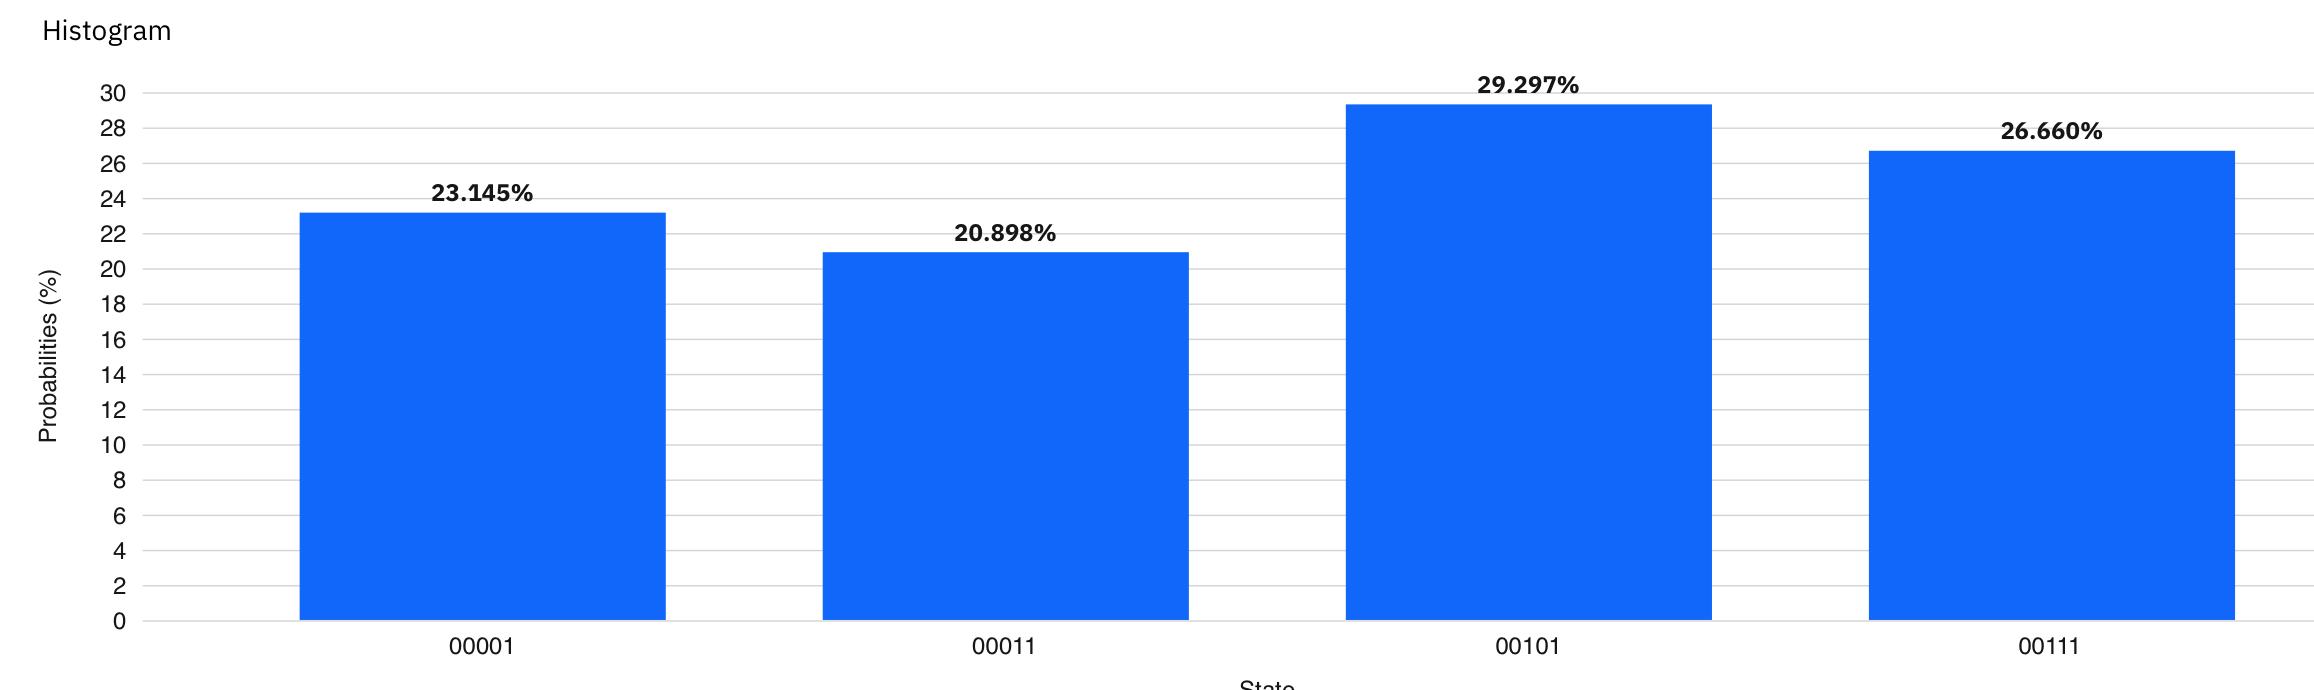
\includegraphics[width=\linewidth]{Circuits/Deutsch-Jozsa-result.png}
            \caption{Result of Balanced Function}
        \end{figure}
        \begin{figure}
            \centering
            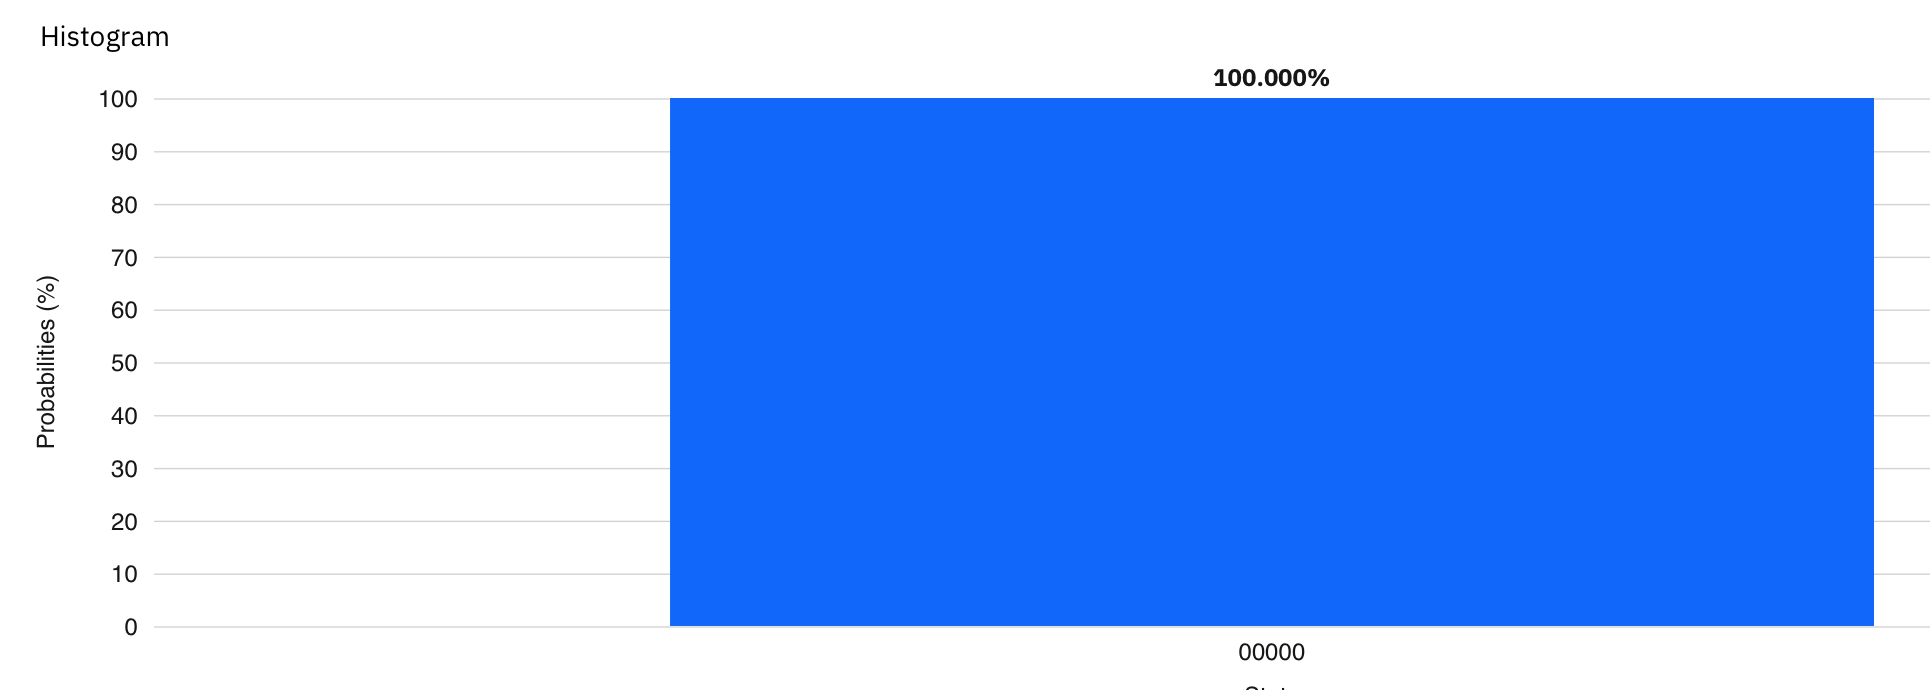
\includegraphics[width=0.6\linewidth]{Circuits/Deutsch-Jozsa-result2.png}
            \caption{Result of Constant Function}
        \end{figure}
    \subsection{Grover Search algorithm}
        This algorithm looks the 
        \begin{figure}[ht]
            \centering
            \begin{minipage}{0.35\linewidth}
                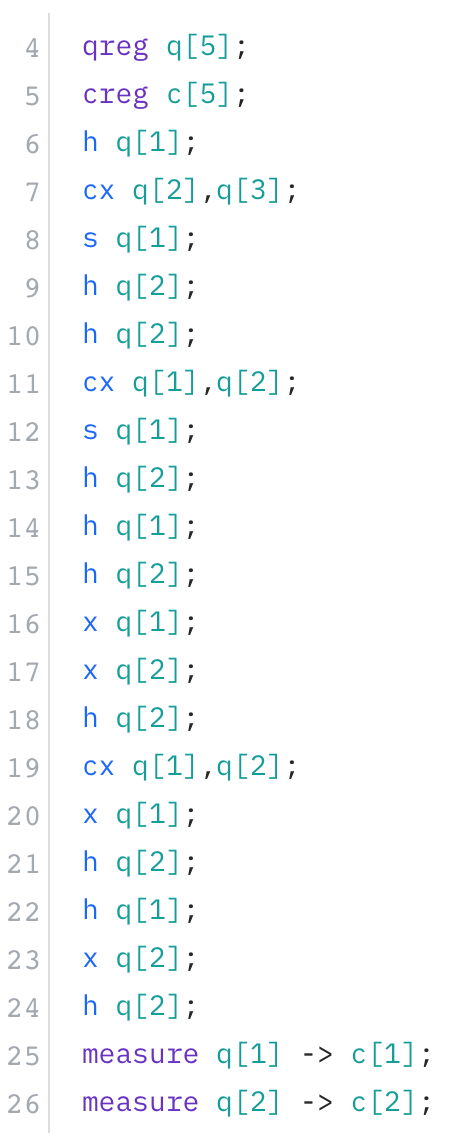
\includegraphics[width=\linewidth]{Circuits/grover-code.png}
            \end{minipage}%
            \begin{minipage}{0.65\linewidth}
                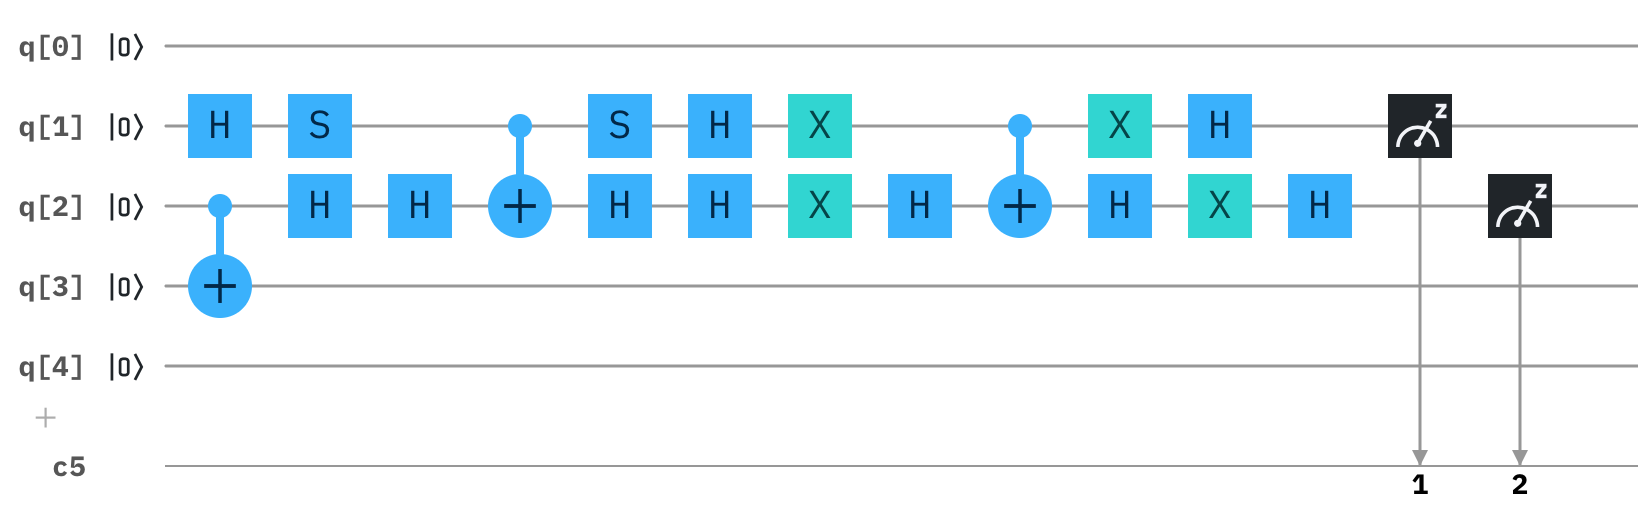
\includegraphics[width=\linewidth]{Circuits/grover.png}
            \end{minipage}
            \caption{Grover Search algorithm}
        \end{figure}
    
\section{Conclusion}
    As of now, quantum computing does not have many general purpose abilities. While the IBM quantum computer is fascinating to experiment with and prove certain results, its computational power is quite limited. The IBM Q software was designed to allow academics and engineers to test circuits on an actual quantum computer and further software development with quantum algorithms. While the current IBM quantum computer does not provide practical benefits, it still benefits our understanding of quantum computation for when quantum computers become more accessible. IBM's software is easy to approach and use while still allowing for more complicated research and application. It was really rewarding to learn about and apply circuits from class to a real quantum computer. This paper only skims the surface of the possibilities of this software and only further research and testing will reveal the full capability of IBM's quantum software.
    \\
    \smallskip
    \\
    In order to distinguish between states and make calculations, a two level system is required. While bits in classical computing can be easily flipped and distinguished, physical qubits are extremely volatile and will rapidly decay their energy into the environment. The current most promising method of maintaining a two level system with superconducting qubits is to keep them at extremely low temperatures. For example, the IBM Quantum Experience keeps its superconducting qubits at 15 milliKelvin in order to reduce ambient heat and noise from interfering with the system. Despite this, our current technology and understanding only allows qubits to be maintained at an excited state for a small number of microseconds. Thus any quantum computation that takes longer than a small number of microseconds will become meaningless. This severely limits the current potential of quantum computers in tackling practical problems.
    \\
    \smallskip
    \\
    
    


\newpage

\section{Appendix}
\subsection{Qiskit}
        Qiskit is a framework developed around QASM to make it possible to work with IBM Q from a console. For the purposes of this project we didn't create any Qiskit files but, it would be very useful for future research. This framework can be installed as a Python library through the pip package manager. When a user inputs their API key for the IBM Q software they can send any QASM circuit to one of the backend servers for processing. The server responds with a dictionary of each possible qubit state and the number of runs that resulted in that state. This interface allows for more nuanced work and allows a user to save configuration and circuit settings between queries. For the average user Qiskit adds a lot of unnecessary complexity and code to the process of drawing and testing a quantum circuit but, for researchers and engineers it allows for more flexible configurations and setups for testing quantum circuitry.

\end{document}

